% !TEX root = ../script.tex
\section{Байесовская теория принятия решений}

\subsection{Задача выбора решающего правила}

Будем рассматривать задачу статистического оценивания на основе выборки данных: заданы
параметр $\theta \in \Theta$, определяющий распределение данных, 
$X$ --- наблюдения, на основе которых нужно принять решение $\delta(X)$
и риск $l(\theta, \delta(X))$, который штрафует
за решение $\delta(X)$ при заданном параметре $\theta$.
Необходимо найти такое решающее правило $\delta(X)$,
которое будет минимизировать риск $l(\theta, \delta(X))$.

\begin{example}
Рассмотрим следующий естественный пример.
Пусть задача состоит в оценке параметра $\theta$, то есть
$\delta(X) = \hat{\theta}(X)$, а риск --- квадратичный,
\[
l(\theta, \delta(X)) = (\theta - \delta(X))^2.
\]
\end{example}

Отметим, что мы еще не до конца сформировали нашу задачу, 
так как природа модели у нас вероятностная,
и $l(\theta, \delta(X))$ --- случайная величина.

\subsection{Выбор решающего правила с использованием среднего риска}

В классическом подходе к статистическому оцениванию обычно 
используют вероятстный или средний риск:
\[
R(\theta, \delta) = \bbE_{\theta} l(\theta, \delta(X)) 
= \int l(\theta, \delta(X)) p(X| \theta) dX,
\]
то есть мы усредняем риск по всем выборкам $X$, сгенерированным из распределения $p(X| \theta)$.

Теперь мы получим детерминированный --- при заданном $\theta$ --- 
средний риск.
Однако мы все еще не можем однозначно сравнить два решающих правила
$R(\theta, \delta_1)$ и $R(\theta, \delta_2)$.
Чтобы понять в чем проблема, достаточно посмотреть на рисунок~\ref{fig:risk_comparison}: в большинстве случаев нельзя сказать, какое решение равномерно лучше другого решения.
В примере на рисунке видно, что для всех $\theta$ $R(\theta, \delta_1) \leq R(\theta, \delta_2)$, однако нельзя так же сравнить решающие правила 
$\delta_1$ и $\delta_3$: для каких-то $\theta$ лучше будет использовать 
$\delta_1$, а для каких-то --- наоборот.

\begin{figure}[h!]
\centering
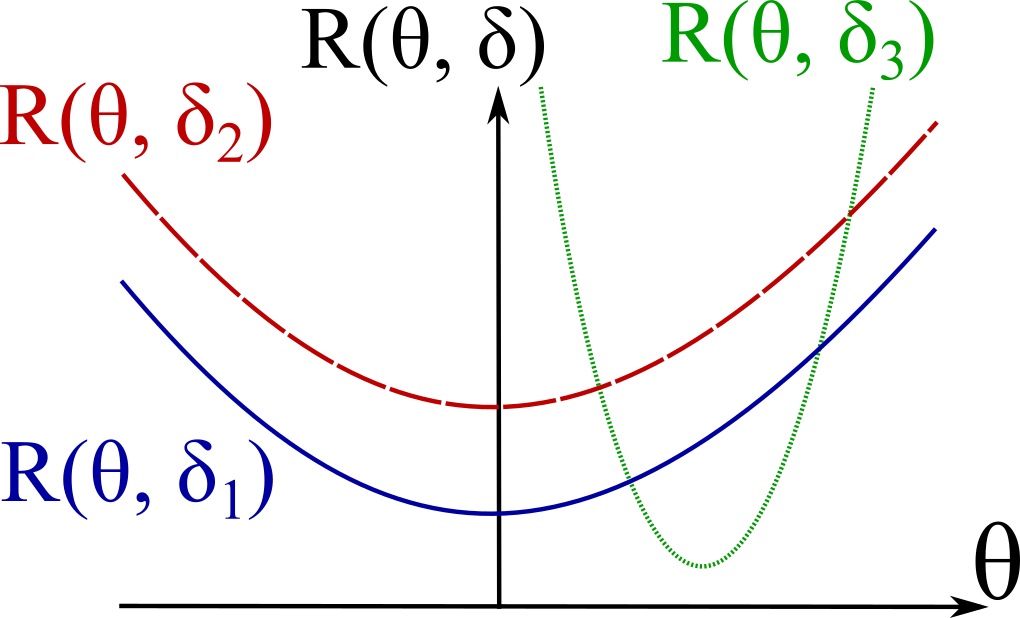
\includegraphics[width=0.5\textwidth]{figures/risk_comparison.png}
\caption{Сравнение средних рисков для решающих правил 
$\delta_1$, $\delta_2$, $\delta_3$}
\label{fig:risk_comparison}
\end{figure}

Перечислим подходы, которые используются для сравнения решающих правил с использованием среднего риска в классической математической статистике:
\begin{itemize}
	\item Решающее правило $\delta$ будет \emph{эффективным}, если для любого другого решающего правила $\delta'$ выполнено, что 
	\[
	\forall \theta \in \Theta: R(\theta, \delta) \leq R(\theta, \delta').
	\]
	Как мы увидели выше, таких решающие правила если и встречаются, то в очень ограниченном классе задач. Однако, можно говорить не про эффективность в целом, а про эффективность в более узком смысле.
	\item Естественно \emph{ограничить класс решающих правил}, в котором мы будем искать целевое решающее правило. Например, в задаче оценки параметра мы можем искать только решающие правила, которые дают несмещенную оценку: $\bbE_{\theta} \hat{\theta}(X) = \theta.$ В классе несмещенных оценок для некоторых классов статистических моделей эффективные оценки существуют. В частности, существует классическая вероятностная теория про эффективность оценок достаточных статистик в экспоненциальном классе распределений.
	\item Решающее правило $\delta$ будет \emph{минимаксно эффективным},
	\index{минимаксный подход}
	если 
	\[
	\forall \delta' \ne \delta: \sup_{\theta} R(\theta, \delta) \leq 
	\sup_{\theta} R(\theta, \delta').
	\]
	Такой подход сводит сравнение средних рисков к сравнению чисел,
	которые агрегируют информацию про средние риски.
	Однако, минимаксный подход кажется излишне консервативным в большинстве случаев. Нас редко интересует то, насколько хорошо все работает в худшем случае, обычно мы хотим оценить качество работы решающего правила в среднем.
\end{itemize}

\subsection{Байесовская теория принятия решений}

Другая естественная идея, возникающая в теории принятия решений,
--- взвесить средний риск с помощью некоторой функции $\pi(\theta)$.
Тогда мы опять сведем задачу сравнения двух решающих правил к задаче сравнения двух чисел $\int R(\theta, \delta) \pi(\theta) d\theta$.

Естественный кандидат на роль такой функции --- априорное распределение на $\theta$.
Таким образом Байесовский подход может быть естественным образом использован в теории принятия решений.

Однако, посмотрим на нее с еще одной стороны.
Введем апостериорный риск:
\[
\rho(\pi, \delta(X)) = \int_{\Theta} l(\theta, \delta(X)) p(\theta| X) d\theta.
\]
Решением, которое минимизирует апостериорный риск будем называть Байесовским решением $\delta^*(X)$.
Как и раньше, для выбора $\delta^*(X)$ нет необходимости уметь считать $p(X)$, достаточно уметь считать $p(x| \theta) \pi(\theta) \propto p(\theta | X)$.

\begin{example}
Получим Байесовское решение для квадратичной функции потерь $l(\theta, \delta(X)) = (\theta - \delta(X))^2$.
Апостериорный риск имеет вид:
\[
\rho(\pi, \delta(X)) = \int_{\Theta} (\theta - \delta(X))^2 p(\theta| X) d\theta = \delta(X)^2 - 2 \delta(X) \int \theta p(\theta | X) d\theta +
\int \theta^2 p(\theta | X) d \theta.
\]
Последний член от $\delta(X)$ не зависит.
Дифференцируя разность первых двух по $\delta(X)$, получаем необходимое условие локального экстремума:
\[
\frac{\partial\rho(\pi, \delta(X))}{\partial \delta(X)} = 2 \delta(X) - 2 \int \theta p(\theta | X) d\theta = 0.
\]
Следовательно, Байесовское решение имеет вид:
\[
\delta^*(X) = \int \theta p(\theta | X) d\theta,
\]
то есть оно совпадает с апостериорным средним.
Если мы возьмем $l_1$ функцию потерь $l(\theta, \delta(X)) = \| \theta - \delta(X) \|$, то получим, что Байесовское решающее правило --- медиана апостериорного распределения.

\end{example}

Определим теперь Байесовское решающее правило, как функцию $\delta_\pi(X)$, которая минимизирует
\[
r(\pi, \delta) = \int R(\theta, \delta) \pi(\theta) d\theta,
\]
где $R(\theta, \delta)$ --- средний риск.
Таким образом мы усреднили средний риск по априорному распределению $\theta$.

Назовем $r(\pi) = r(\pi, \delta_\pi)$.
Мы можем интерпертировать его и с более Байесовской точки зрения.
Действительно, 
\begin{align*}
r(\pi, \delta) &= \int \int l(\theta, \delta(X)) p(X | \theta) dx \, \pi(\theta) d\theta = \\
&= \int \int l(\theta, \delta(X)) p(\theta | X) d\theta p(X) dX = \\
&= \int \rho(X, \pi) p(X) dX.
\end{align*}
Таким образом, $r(\pi, \delta)$ --- усреднение апостериорного риска по маргинальному распределению $p(X)$.
Таким образом, Байесовское решающее правило --- совокупность Байесовских решений для всех $X$.

Отметим, что такой подход может быть использован для получения минимаксных оценок, так как во многих случаях мы можем получить Байесовское решающее правило в явном виде.

\subsection{Проблемы несмещенных оценок}

Приведем в завершении этого раздела несколько классических примеров задачи статистического оценивания, демонстрирующих неэффективность несмещенных оценок.

\begin{example}[Регрессия к среднему]
Рассмотрим следующий пример.
Пусть $x$ --- рост матери, а $y$ --- рост дочери.
$x$ и $y$ --- случайные величины из многомерного нормального распределения:
\[
\begin{pmatrix}
x \\ y
\end{pmatrix} \sim
\mathcal{N}
\left( 
\begin{pmatrix}
\mu_1 \\ \mu_2
\end{pmatrix},
\begin{pmatrix}
\sigma^2 & \rho \\ \rho & \sigma^2
\end{pmatrix}
\right).
\]
Возьмем $\mu_1 = \mu_2 = 160 \text{см}$, $\bbV x = \bbV y = \sigma^2 = 1$ и $\rho = 0.5$.

Тогда 
\[
\bbE (y | x) = \mu_2 + \rho (x - \mu_1)
\]

Следовательно,
\begin{align*}
\bbE_y \bbE (y | x) &= 160 + 0.5 (\bbE_y x - 160) = \\
                    &= 160 + 0.5 (160 + 0.5(y - 160) - 160) = \\
                    &= 160 + 0.25 (y - 160)
\end{align*}

Ясно, что такая оценка не совпадает с $y$ и, более того, не является несмещенной.
В то же время математическое ожидание для несмещенной оценки будет иметь вид:
\[
\hat{y} = 160 + 2 (x - 160).
\]
Такая несмещенная оценка противоречит здравому смыслу ---
получается, что дочка должна в среднем сильнее отклоняться от среднего роста, чем мать.
На практике наблюдается обратная ситуация, которую описал еще пионер математической статистики и автор термина регрессия Фрэнсис Гальтон:
обычно дети ближе к среднему росту, если рост их родителей аномально высокий.
Название феномена \emph{регрессия к среднему} и привело к появлению термина регрессия.
% http://ww2.amstat.org/publications/jse/v9n3/stanton.html

\end{example}

\begin{example}[Два орла подряд]
Пусть мы подбросили монету $\sS$ раз, 
причем число орлов распределено биномиально $B(\sS, \theta)$.
Мы наблюдаем $r$ орлов и хотим оценить $\theta^2$,
вероятность наблюдения двух орлов подряд.
В таком случае мы можем получить эффективную несмещенную оценку --- несмещенную оценку с минимальной дисперсией:
\index{эффективная оценка}
\index{несмещенная оценка}
\[
\hat{\theta^2} = \frac{r(r - 1)}{n (n - 1)}.
\]

Получается, что для $r = 1$ такая оценка равна нулю.
То есть, вероятность получить два орла подряд равна нулю.
Существует ли оценка, свободная от этого недостатка, и как ее получить?
\end{example}

\begin{example}[Парадокс Штайна]
\index{парадокс Штайна}
Рассмотрим $\vecX = \{x_1, \ldots, x_{\pD}\}$.
Каждый $x_i \sim \mathcal{N}(\theta_i, \sigma^2)$.
Задача состоит в оценке вектора параметров $\vecT = \{\theta_1, \ldots, \theta_{\pD}\}$.
Функция потерь квадратичная, $l(\vecT, \hat{\vecT}(\vecX)) = \bbE \|\vecT - \hat{\vecT}\|^2$.

Естественная несмещенная оценка в данном случае совпадает с оценкой максимума правдподобия, $\hat{\vecT}_{MLE} = \vecX$.

Однако, оказывается, что такая оценка не является эффективной.
Рассмотрим, например, оценку Джеймса-Штайна:
\[
\hat{\vecT}_{JS} = \left(1 - \frac{(\pD - 2) \sigma^2}{\|\vecX\|^2} \right) \vecX.
\]
Для $\pD \geq 3$ такая оценка оказывается эффективнее, чем оценка максимума правдоподобия.
Однако и она не будет самой эффективной.
Оценка Джеймса-Штайна с параметром $\boldsymbol{\nu}$ оказывается еще более эффективной для $\pD \geq 4$:
\[
\hat{\vecT}_{JS\boldsymbol{\nu}} = \left(1 - \frac{(\pD - 3) \sigma^2}{\|\vecX - \boldsymbol{\nu}\|^2} \right) (\vecX - \boldsymbol{\nu}) + \boldsymbol{\nu}.
\]

В частности, она более эффективна, чем Байесовская оценка 

\[
\hat{\vecT}_{JS\boldsymbol{\nu}+} = \left(1 - \frac{(\pD - 3) \sigma^2}{\|\vecX - \boldsymbol{\nu}\|^2} \right)^+ (\vecX - \boldsymbol{\nu}) + \boldsymbol{\nu}.
\]
\end{example}


%TODO Bias-variance tradeoff?